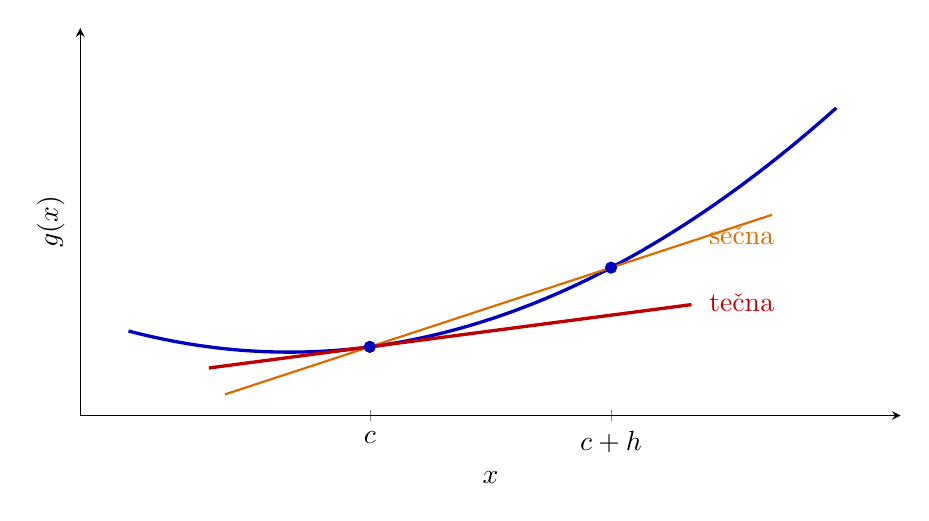
\begin{tikzpicture}
    \begin{axis}[
        width=12cm,height=6.5cm,
        xmin=-0.3,xmax=4.8,ymin=-0.3,ymax=5.2,
        axis lines=left,xlabel={$x$},ylabel={$g(x)$},
        xtick={1.5,3},xticklabels={$c$,$c+h$},
        ytick=\empty,
        label style={font=\normalsize},
        tick label style={font=\normalsize},
        every node/.style={font=\normalsize},
        clip=false
    ]
        \addplot[blue!75!black,very thick,domain=0:4.4,samples=100]
            {0.3*(x-1)^2+0.6};
        % Sečna prochází body (c,g(c))=(1.5,0.675) a
        % (c+h,g(c+h))=(3,1.8); její směrnice je 0.75.
        \addplot[orange!85!black,thick,domain=0.6:4]
            {0.75*x-0.45};
        % Derivace g'(x)=0.6(x-1), takže tečna v c=1.5 má
        % směrnici 0.3 a rovnici y=0.3x+0.225.
        \addplot[red!75!black,very thick,domain=0.5:3.5]
            {0.3*x+0.225};
        \addplot[only marks,mark=*,blue!75!black]
            coordinates{(1.5,0.675)(3,1.8)};
        \node[orange!85!black,anchor=west] at (axis cs:3.55,2.25){sečna};
        \node[red!75!black,anchor=west] at (axis cs:3.55,1.30){tečna};
    \end{axis}
\end{tikzpicture}
